%______________________________________________________declaration package__________________________________________
\documentclass[12pt,a4paper]{article}
\usepackage[french]{babel} 
\usepackage[utf8]{inputenc}
\usepackage[T1]{fontenc}
\usepackage{amsmath,amsfonts,amssymb}
\usepackage{makeidx}
\usepackage{graphicx}
\usepackage{wrapfig}
\usepackage{xcolor}
\usepackage{listings}
\usepackage{float}
\usepackage[top=2cm, bottom=2cm, left=2cm, right=2cm]{geometry}
\usepackage{titlesec}
\usepackage{url}
\usepackage{subfigure}
\usepackage{textcomp}

\definecolor{darkWhite}{rgb}{0.94,0.94,0.94}

\lstset{
  aboveskip=3mm,
  belowskip=-2mm,
  backgroundcolor=\color{darkWhite},
  basicstyle=\footnotesize,
  breakatwhitespace=false,
  breaklines=true,
  captionpos=b,
  commentstyle=\color{red},
  deletekeywords={...},
  escapeinside={\%*}{*)},
  extendedchars=true,
  framexleftmargin=16pt,
  framextopmargin=3pt,
  framexbottommargin=6pt,
  frame=tb,
  keepspaces=true,
  keywordstyle=\color{blue},
  language=c,
  literate=
  {²}{{\textsuperscript{2}}}1
  {⁴}{{\textsuperscript{4}}}1
  {⁶}{{\textsuperscript{6}}}1
  {⁸}{{\textsuperscript{8}}}1
  {€}{{\euro{}}}1
  {é}{{\'e}}1
  {è}{{\`{e}}}1
  {ê}{{\^{e}}}1
  {ë}{{\¨{e}}}1
  {É}{{\'{E}}}1
  {Ê}{{\^{E}}}1
  {û}{{\^{u}}}1
  {ù}{{\`{u}}}1
  {â}{{\^{a}}}1
  {à}{{\`{a}}}1
  {á}{{\'{a}}}1
  {ã}{{\~{a}}}1
  {Á}{{\'{A}}}1
  {Â}{{\^{A}}}1
  {Ã}{{\~{A}}}1
  {ç}{{\c{c}}}1
  {Ç}{{\c{C}}}1
  {õ}{{\~{o}}}1
  {ó}{{\'{o}}}1
  {ô}{{\^{o}}}1
  {Õ}{{\~{O}}}1
  {Ó}{{\'{O}}}1
  {Ô}{{\^{O}}}1
  {î}{{\^{i}}}1
  {Î}{{\^{I}}}1
  {í}{{\'{i}}}1
  {Í}{{\~{Í}}}1,
  morekeywords={*,...},
  numbers=left,
  numbersep=10pt,
  numberstyle=\tiny\color{black},
  rulecolor=\color{black},
  showspaces=false,
  showstringspaces=false,
  showtabs=false,
  stepnumber=1,
  stringstyle=\color{gray},
  tabsize=4,
  title=\lstname,
}

%_________________________________debut du doc________________________________________

\begin{document}

%_________________________________page de garde_______________________________________

\begin{titlepage}
\newcommand{\HRule}{\rule{\linewidth}{0.1mm}}
\center


\includegraphics[scale=0.4]{logo.png} \\[0.2cm]

\includegraphics[scale=0.7]{CHPS_logo.png} \\[1.5cm]

\HRule 
{ \huge \bfseries Allocateur Mémoire \\ AISE
  \\[0.15cm] }
\HRule \\[1.5cm]

\textbf{Réalisé par :} \\ Hamza ELBARAGHI \\ Sofiane BOUZAHER \\ Atef DORAI 
\\[1cm]
\today \\ [1cm]
\end{titlepage}


%______________________________________sommmaire_______________________________________

\renewcommand*\contentsname{Sommaire}
\tableofcontents

\pagebreak

%___________________________contenu du rapport___________________________________________

\section{Introduction}
Le but de ce projet est de développer un allocateur mémoire capable d'être lancé en
remplacement de l’allocateur système pour n’importe quel type d’application ou de
bibliothèque. chaque Allocateur de memoire contient les fonctions suivantes :

\subsection{malloc}
La fonction standard \textbf{malloc} a comme paramétre la taille de memoire à alloué en bytes  et comme retour un pointeur vers la zone allouée ou 0 si la taille entré est 0. En notant que la memoire alloué n'est pas initialisé. 

\subsection{calloc}
La fonction standard \textbf{calloc ()} prend en entrée deux parametres 'nmemb' et 'size' pour allouer de la mémoire un tableau de 'nmemb' éléments et de taille 'size' octets chacun ,et 
renvoie un pointeur sur la mémoire allouée on dirait malloc mais avec un mise à zéro de la mémoire. Si nmemb ou size est 0, calloc () renvoie soit NULL, soit une valeur de pointeur unique qui peut plus tard réussir entièrement passé à free ().

\subsection{realloc}

La fonction standard \textbf{realloc ()} prend comme parametres d'entreé un 'pointeur' et un 'size' afin de modifier la taille du bloc de mémoire pointé par 'ptr' en 'size' octets.
 Si la nouvelle taille est plus grande que l'ancienne taille, la mémoire ajoutée ne sera pas initialisé. Si ptr est NULL, alors l'appel est équivalent à malloc (size), si la size est égale à zéro et ptr n'est pas NULL, alors l'appel est équivalent à free(ptr). Si la zone pointée a été déplacée, un free (ptr) est effectué.

\subsection{free}
la function standard \textbf{free} libere l'espace memoire , un appel précédent à malloc (),calloc () ou realloc () est obligatoire pour retourne le ptr qui sera utiliser par free. Si ptr est NULL, aucune opération n'est effectuée.

\section{Déscription du code}
\subsection {Recyclage de blocs et metadonnées}

 
\begin{figure}[htp]
    \centering
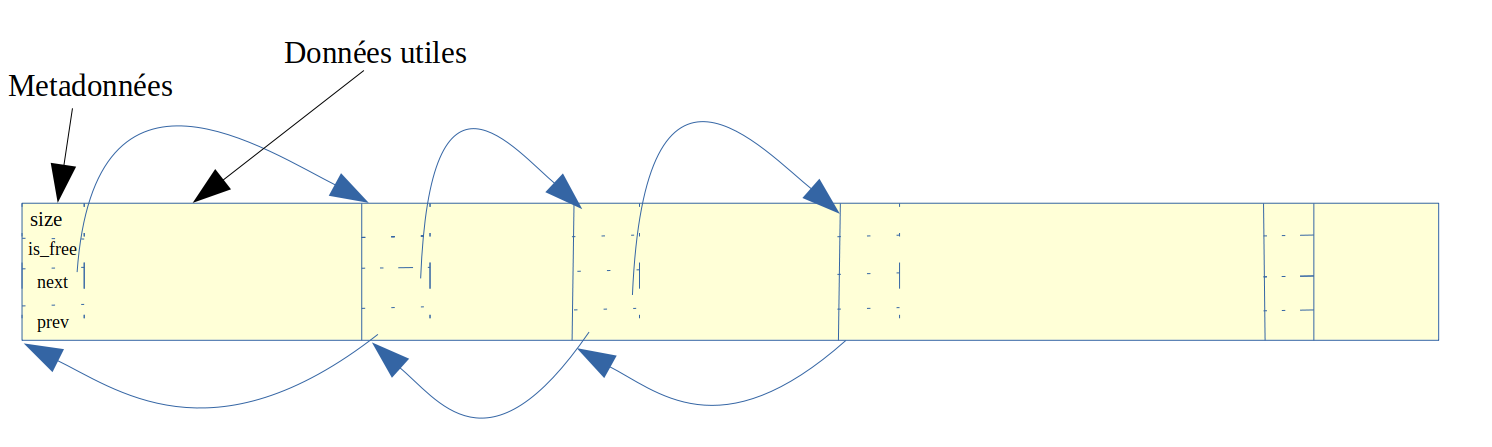
\includegraphics[width=12cm]{struct.png}    
   \caption[Recyclag de blocs]{Recyclage de blocs}
\end{figure}





Pour notre implémentation, nous avons choisi une structure de donnée contenant les données utiles pour les blocs alloués/désalloulés, à savoir : la taille du bloc, son état (alloué ou désalloué), un pointeur vers le bloc suivant, et un poineur vers le bloc précédent.


\begin{figure}[htp]
    \centering
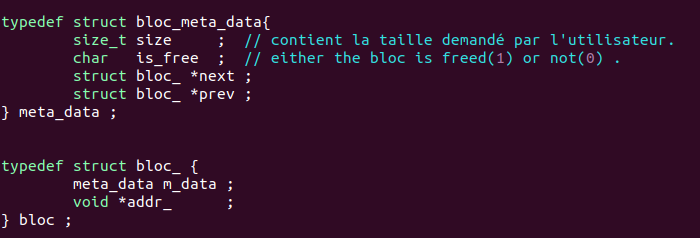
\includegraphics[width=12cm]{struct1.png}    
   \caption[Structure de donnée]{Structure metadonnées}
\end{figure}


Metadonnées : Les métadonnées représentent des informations sur le bloc alloué, et sur le bloc suivant et précédant; cela permet d'optimiser le nombre d'appel à la fonction mmap : un appel au malloc ne fait  pas nécessairement un appel à mmap.


Recyclage de blocs :
\begin{itemize} 

	\item \textbf {Première allocation    :} 
		première mapping = appel mmap d'une page de 4KB

	\item \textbf {Prochaines allocations :} 
		dépend de la taille demandée :

\begin{itemize}
	\item 		 Si la taille demandée est supérieure à 4KB (taille d'une page) => un autre appel à mmap est nécessaite
 
	\item 		 Si la taille demandée est inférieur à 4KB  => On parcours les pages déjà aloués et on cherche le premier bloc free et dont la size est supérieure ou égale à la taille demandé, on récupère la zone suffisante dans ce bloc, et on modifie les données de métadonnées .  
\end{itemize}
\item \textbf {Reallocation :}


	Pour réallouer une zone, on vérifie si le bloc suivant (s'il existe) est suffisant, si c'est le cas on merge les deux blocs et on modifier les informations sur les métadonnées des deux blocs, sinon on fait appel à malloc, et on copie les données initiales dans l'adresse retourné.
\item \textbf {Free :}


	On modifie les métadonnées de l'adresse à libéré ; on met is\textunderscore free = 1 pour signaler que cet zone est libre pour les prochaines malloc .
	
	En plus, on merge avec le bloc suivant s'il est free pour construire un seul bloc free, de meme pour le bloc précédent .
	
\item \textbf {Alignement :}

	
	Avant d'allouer un blocon aligne d'abord la taille demandé en plus de la taille des métadonnées ( sizeof(meta\textunderscore data) ) sur le mot machine pour optimiser les accès mémoire en lecture et écriture.


\item \textbf {Multithreading :}
	
	
	Pour une application qui lance plusieurs threads, et chaque thread essaye d'allouer une zone mémoire, il faudra protéger les zones allouer pour chaque thread, pour cela nous avons ajouter une mutex dans notre implémentation, et à chaque fois on accéde à une section critique on la protége avec les deux fonctions : pthread\textunderscore mutex\textunderscore lock et   pthread\textunderscore mutex\textunderscore unlock 


\end{itemize}



\section{Les tests}

Pour tester notre bibliothèque nous avons imlémenté une boucle dont on fait appel à  malloc/realloc/free et on mesure on le temps écoulé : 

Premièrement une boucle de plusieurs malloc de tailles aléatoires, puis une autre boucle pour free des zones aléatoires parmi les zones alloués précédément. et en suite une boucle pour réalloc .






%____________________________________________conclusion_________________________________________________________

\section{Conclusion}

Nous avons implémenté notre propre bibliothèque d'allocation mémoire en utilisant le principe de recyclage de bloc, et la méthode : implicit free list pour allouer un bloc parmi les blocs désalloués, ainsi qu'on a implémenté pour la fonction free une technique qui permet de rassembler les free zones qui sont succcessives, en plus on a protégé les zones critique par des mutex pour mettre notre bibliothèque thread-safe .

Nous pouvons améliorer notre implémentation, par exemple en adoptant la méthode : best fit free list qui permet de chercher pour une allocation donnée le bloc optimal, ou la méthode segregated free list qui cherche le bloc optimal parmi une liste de blocs triés par tailles, ce qui permet de minimiser le temps de recherche de blocs .


Par contre, nous avons rencontrés des difficultés au niveau de l'intreposition de notre bibiothèque avec la libc .

\pagebreak


%__________________________________________biblio______________________________________________________________ 

\nocite{*} 

\bibliography{mybib}
\bibliographystyle{plain}


\end{document}
%______________________________________________________declaration package__________________________________________
\documentclass[12pt,a4paper]{article}
\usepackage[french]{babel} 
\usepackage[utf8]{inputenc}
\usepackage[T1]{fontenc}
\usepackage{amsmath,amsfonts,amssymb}
\usepackage{makeidx}
\usepackage{graphicx}
\usepackage{wrapfig}
\usepackage{xcolor}
\usepackage{listings}
